%=======================================================================
\section{Performance Evaluation}
\label{sec:performance}
%=======================================================================

We evaluate SENTINEL with the simulator released with this paper\footnote{\url{https://github.com/tanzimulalam/Quantum_SAGIN_AoII_Updated_Simulation}, tag \texttt{v2.2-manuscript}; the script \texttt{scripts/reproduce\_all.sh} regenerates every table and figure.}
under the parameters of Table~\ref{tab:simulation_parameters}, which are the values used for every figure. Each
configuration runs for 60{,}000 slots of 10~ms, ten minutes of network time, on 30 independent seeds; the policies of
one seed share its topology, source trajectories, fading, and disruption realization, so all comparisons are paired.
We report medians with interquartile ranges, because a few seeds contain long non-line-of-sight passes that dominate
means; means with 95\% confidence intervals, the raw per-seed results, and the paired test tables are in the
repository.

\begin{table}[t]
\centering
\caption{Simulation Parameters (values used for all figures)}
\label{tab:simulation_parameters}
\scriptsize
\renewcommand{\arraystretch}{1.12}
\begin{tabular}{p{0.46\columnwidth} p{0.46\columnwidth}}
\hline
\textbf{Parameter} & \textbf{Value} \\
\hline
\multicolumn{2}{l}{\emph{Network}} \\
Number of UEs & $\{5,10,15,20\}$; up to 100 in Sec.~VI-D \\
BSs / satellite serving slots & 2 / 2 (topology study: 0 to 3 each) \\
Area; BS height; UE height & $20\times20$~km$^2$; 25~m; 1.5~m \\
Satellite passes & Starlink TLE snapshot, SGP4, MTSU site (35.85$^\circ$N, 86.39$^\circ$W); min.\ elevation $25^\circ$ \\
Domains $K$ & 2 (one BS each; satellites shared) \\
\hline
\multicolumn{2}{l}{\emph{Channel and resources}} \\
UE transmit power & 23~dBm \\
UE--BS link & 3.5~GHz, 20~MHz, $-147.55+20\log_{10}f+26\log_{10}d+6$~dB, BS gain 15~dBi, NF 7~dB \\
UE--SAT link & 12~GHz, 50~MHz, free space $+1$~dB, gains 30 $+$ 30~dBi, NF 9~dB \\
NTN large-scale model & TR~38.811 suburban (LOS prob., clutter, shadow fading per pass); atm.\ $0.5$~dB$/\sin V$ \\
Bandwidth levels $\bar\beta^q_m$ ($Q_m=3$) & $\{2.5,5,10\}$~MHz, $\Delta_\beta=2.5$~MHz \\
Spectral-efficiency cap & 6 (BS), 4 (SAT) bit/s/Hz \\
\hline
\multicolumn{2}{l}{\emph{Source and AoII}} \\
Source states; transition matrix & 4; birth--death, self-transition $\mathcal{U}[0.90,0.99]$ per UE \\
Distortion; AoII budget $\Delta^{II,\max}_i$ & $|x-\hat x|$; 10 \\
Update periods ($H_i=4$); slot; packet & $\{5,10,20,50\}$ slots; 10~ms; 20~kbit \\
\hline
\multicolumn{2}{l}{\emph{Disruption}} \\
Scenario set ($L=5$) & nominal; deep shadowing 12~dB for 30 slots; handover of each SAT (20 slots); joint loss (30 slots) \\
Realized process (per 1~s interval) & TR~38.811 state per pass; shadowing event per UE--SAT link w.p.\ 0.07; handover failure per SAT w.p.\ 0.03; natural handovers \\
Link-failure handling (all policies) & node blocked after 60 failed slots, for 6~s or until its next handover; SENTINEL re-solves \\
\hline
\multicolumn{2}{l}{\emph{Solver}} \\
Formulation & compact dual, $\kappa=4$, $T=6$ outer iterations, $\sigma=2$ \\
Local solver & XY-QAOA, depth 1, 512 shots, COBYLA 40 it.\ ($\le 26$ qubits); one-hot annealing otherwise \\
ADMM $\varrho_0$, tolerance, rounds & scaled to cost spread, $10^{-2}$, 20 \\
Re-solve & on visibility change, on link failure, at least every 30~s \\
Quantum backend & Qiskit Aer~\cite{Qiskit2024}; FakeTorino / FakeFez; \texttt{ibm\_kingston}, \texttt{ibm\_fez} \\
\hline
\end{tabular}
\end{table}

\textbf{Baselines.} \emph{Random} transmits with probability 0.1 per slot over a uniformly chosen visible node with
equal bandwidth sharing. \emph{AoII threshold} is a state-aware policy that transmits whenever its AoII is positive,
at most once per 5 slots, on the node with the best nominal rate. \emph{Whittle index} is the restless-bandit
scheduler of the AoII literature~\cite{Whittle1988, Kadota2018}: the index of each UE's (source state, estimate, age)
arm is computed numerically per source by relative value iteration on a grid of transmission prices, and every slot
the mismatched UEs are ranked by index and admitted at their best node while the node's shared bandwidth still
delivers every admitted packet; it has the threshold policy's observations and rate cap. \emph{PPO} is an actor-critic
agent~\cite{Schulman2017} that selects, once per orchestration interval, a serving node and an update-period level for
every UE, with invisible or failed nodes masked and equal bandwidth sharing, rewarded with the negative mean AoII of
the interval; it is trained for 5000 episodes per network size on 30 seeds disjoint from the evaluation seeds and
evaluated deterministically on the same episodes as every other policy. \emph{Nominal SENTINEL} runs Algorithm~1
with the nominal scenario alone ($L=1$). \emph{SENTINEL} is the robust schedule with the five-scenario set. \emph{SENTINEL
+ trigger} uses SENTINEL's association and bandwidth with transmissions triggered by the observed mismatch,
rate-capped at the chosen period. Every policy receives the same acknowledgement feedback and applies the same
link-failure rule of Section~III-F. The exact reference for Section~VI-D is the integer linear program
$\mathscr{P}_3$ solved with HiGHS~\cite{HiGHS2018}.

%-----------------------------------------------------------------------
\subsection{AoII Versus Network Size}
\label{sec:ue_sweep}
%-----------------------------------------------------------------------

\begin{figure}[!t]
\centering
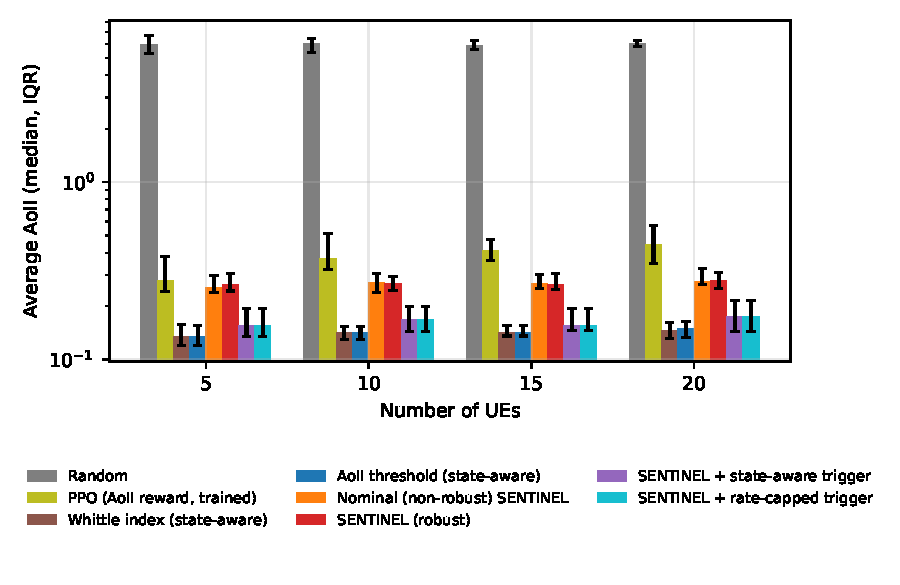
\includegraphics[width=0.86\columnwidth]{figures/ue_sweep_average_aoii_median_disruption_on.pdf}
\caption{Median average AoII (bars) and interquartile range (whiskers) over 30 seeds versus the number of UEs, with
Starlink passes, the TR~38.811 channel, and the stochastic disruption process active.}
\label{fig:ue_sweep}
\end{figure}

Fig.~\ref{fig:ue_sweep} and Table~\ref{tab:tle} give the median average AoII from 5 to 20 UEs. Three groups are
visible. The state-aware per-slot policies, AoII threshold and Whittle index, are lowest at 0.13 to 0.15 and coincide
(Section~VI-C). The SENTINEL schedules, robust and nominal, sit at 0.25 to 0.28 and do not grow with the number of
UEs, because bandwidth levels are dedicated and a re-solve redistributes load as satellites come and go. SENTINEL with
the state-aware trigger lies between the two at 0.155 to 0.175: it keeps the robust association and bandwidth,
transmits only when the estimate is wrong, and thereby raises the informative-update ratio from 0.23 to 0.96 while
retaining the certificate. Random scheduling is at 6; the trained PPO agent matches the nominal schedule at 5 UEs
(0.280 against 0.253), degrades to 0.446 at 20 UEs as its action space grows, routes all traffic to satellites, and,
like SENTINEL, samples without observing the source. Delivery ratios are 0.92 to 0.94 for every policy except random;
the per-slot policies deliver with 2.8 to 3.0~ms of end-to-end latency against 4.7 to 5.8~ms for the SENTINEL
schedules, whose dedicated levels are smaller than an equal share of an otherwise idle node. The satellite tier
carries 73 to 79\% of robust SENTINEL's deliveries and 97 to 98\% of the threshold policy's. Peak AoII is 100 to 400
for every policy and is set by handover interruptions and non-line-of-sight passes rather than by the scheduler. A
20-UE solve used 20 to 58 qubits per domain and the orchestration loop 34 to 223~s of solver time per run.

\begin{table}[!t]
\centering
\caption{Median Average AoII with Starlink Passes and the TR~38.811 Channel (30 seeds, disruption on)}
\label{tab:tle}
\footnotesize
\resizebox{\columnwidth}{!}{%
\begin{tabular}{|c|c|c|c|c|c|c|c|}
\hline
\textbf{UEs} & \textbf{Random} & \textbf{PPO} & \textbf{Whittle} & \textbf{AoII thr.} & \textbf{Nominal} & \textbf{SENTINEL} & \textbf{+ trigger} \\
\hline
5  & 5.94 & 0.280 & 0.134 & 0.134 & 0.253 & 0.265 & 0.155 \\
10 & 6.06 & 0.372 & 0.141 & 0.142 & 0.270 & 0.269 & 0.168 \\
15 & 5.87 & 0.413 & 0.142 & 0.142 & 0.269 & 0.264 & 0.155 \\
20 & 6.05 & 0.446 & 0.146 & 0.149 & 0.276 & 0.278 & 0.175 \\
\hline
\end{tabular}%
}
\end{table}

%-----------------------------------------------------------------------
\subsection{The Certificate and the Value of Robustness}
\label{sec:certificate}
%-----------------------------------------------------------------------

\begin{figure}[!t]
\centering
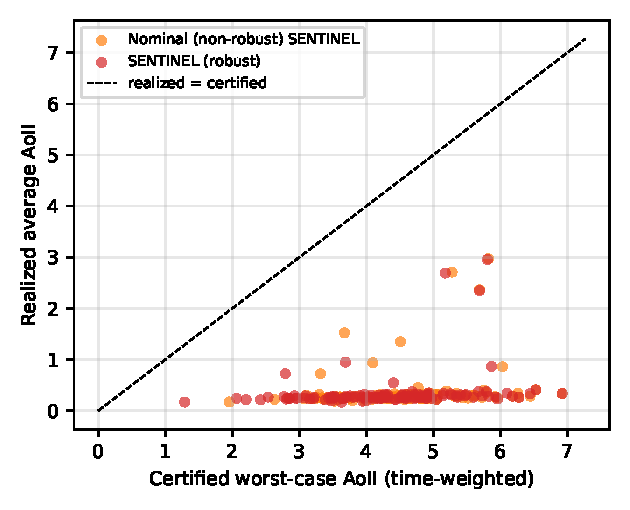
\includegraphics[width=0.78\columnwidth]{figures/certificate_vs_realized.pdf}
\caption{Certified worst-case AoII of each orchestration run against its realized average AoII, robust and nominal
SENTINEL, all sizes and seeds of Fig.~\ref{fig:ue_sweep}. Points below the diagonal stayed within the certificate.}
\label{fig:certificate}
\end{figure}

Fig.~\ref{fig:certificate} plots the certified worst case of every run against the AoII it realized. The realized
average stayed within the certificate in 98.7\% of orchestration epochs for the robust schedule and 98.5\% for the
nominal one; the violations are passes that enter the non-line-of-sight state, whose 17 to 25~dB clutter loss exceeds
the 12~dB deep-shadowing scenario. With a synthetic pass model that produces coverage gaps longer than any scenario
window the figure was 98.0\%, and every violation there was such a gap. The certificate is therefore valid against the
scenario set it was computed from, and the paper states its scope that way.

What the scenario set buys is visible in the certificate, not in the realized AoII. Across the 30 paired seeds the
robust schedule's certified worst case is 2 to 7\% below the nominal schedule's (paired-median ratio 0.93 at 5 UEs to
0.98 at 20 UEs), lower in 67 to 100\% of seeds, with Wilcoxon signed-rank $p\le 9\times10^{-5}$ at every size after
Holm correction. The realized AoII of the two is statistically indistinguishable at every size ($p\ge0.08$), although
the robust mean at 20 UEs is lower, 0.39 against 0.46, because the robust schedule keeps 21 to 27\% of deliveries on
base stations. The gap between SENTINEL with the trigger and the threshold policy, 0.02 to 0.03 in AoII, is small but
significant at every size ($p\le0.013$), and PPO is significantly behind SENTINEL from 10 UEs on.

\begin{figure}[!t]
\centering
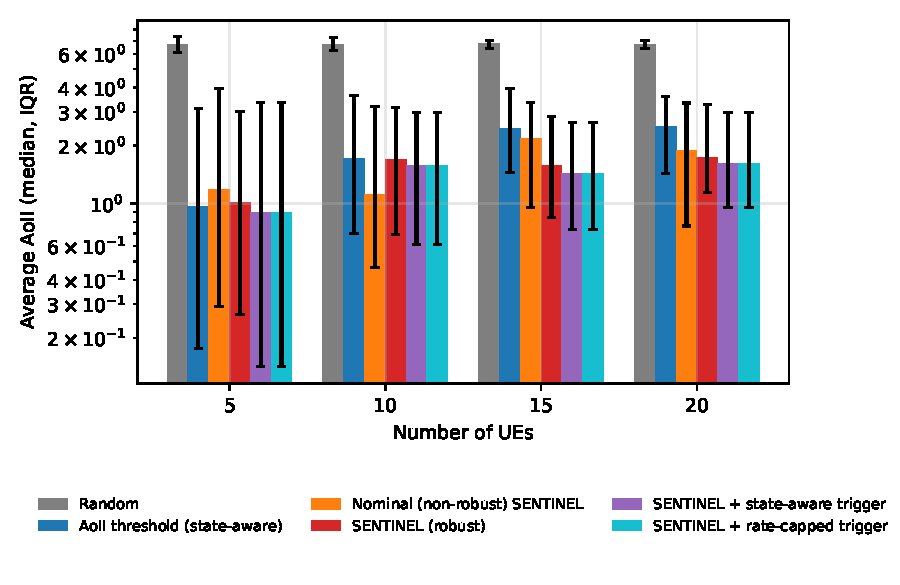
\includegraphics[width=0.86\columnwidth]{figures/noack_ue_sweep_average_aoii_median.pdf}
\caption{Median average AoII (60 seeds) with acknowledgement feedback and link-failure handling disabled for every
policy.}
\label{fig:noack}
\end{figure}

\textbf{Without failure feedback.} Whether the network can react to a dead link matters more than any scheduling
choice. Fig.~\ref{fig:noack} repeats the sweep with the link-failure rule disabled for every policy, on 60 seeds
because the distributions become heavy-tailed. Median AoII rises by an order of magnitude for all policies, the
certificate holds in 87 to 92\% of epochs, and the threshold policy, which concentrates 98\% of its traffic on the best
nominal satellite, ties the SENTINEL schedules at 5 and 10 UEs and falls 25 to 30\% behind SENTINEL with the trigger
at 15 and 20 UEs (Hodges-Lehmann differences $-0.77$ and $-0.71$, Holm-corrected $p=0.023$ and $0.029$), while the
SENTINEL schedules keep 18 to 27\% of deliveries on base stations. Robust and nominal SENTINEL remain
indistinguishable in realized AoII here as well ($p\ge0.41$). The measurable product of the robust scenario set is
thus its lower certificate, obtained in both regimes, and the measurable value of a scheduled base-station share
appears when feedback is absent.

\textbf{Scenario-set size.} To see which scenarios matter, the list was extended by a mild 6~dB shadowing scenario and
truncated to $L=1,\ldots,6$ at 10 UEs. Realized AoII is flat in $L$ (0.265 to 0.278); the certificate and the
base-station hedge move only once the handover of the second shared satellite enters the set, the certified worst
case falling from 4.57 to 4.28 and the satellite share from 0.79 to 0.74 between $L=4$ and $L=5$. The mild scenario
never binds: removing it from the full set leaves the certified worst case of every schedule unchanged on all 30 seeds
at every size, with realized-AoII differences below $10^{-3}$, which is why the paper's scenario set has five members.

%-----------------------------------------------------------------------
\subsection{Topology, the Whittle Index, and Capacity}
\label{sec:topology}
%-----------------------------------------------------------------------

\begin{figure}[!t]
\centering
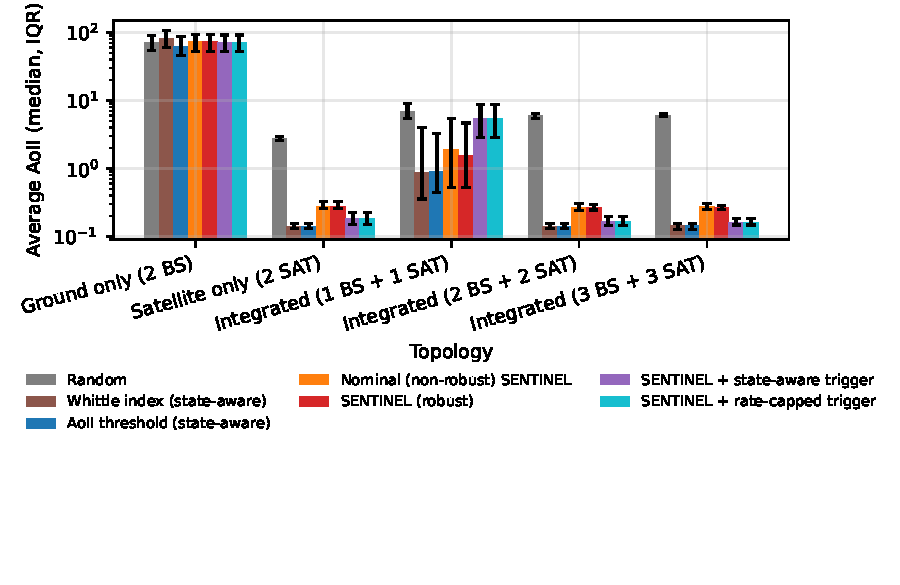
\includegraphics[width=0.86\columnwidth]{figures/topology_average_aoii_median.pdf}
\caption{Median average AoII at 10 UEs for ground-only, satellite-only, and integrated deployments (30 seeds,
disruption on, logarithmic scale).}
\label{fig:topology}
\end{figure}

Fig.~\ref{fig:topology} compares deployments at 10 UEs. Two base stations cover only the UEs within 5 to 7~km of the
$20\times20$~km$^2$ area, so ground-only monitoring fails for every policy (median AoII 63 to 81). Two satellite
serving slots alone bring the per-slot policies to 0.14 and the SENTINEL schedules to 0.18 to 0.28, and the
integrated $2+2$ and $3+3$ deployments are the best for every policy, with SENTINEL routing 26 to 36\% of its
deliveries to base stations. The one deployment in which the SENTINEL schedules are clearly worse than the per-slot
policies is a single base station with a single satellite slot (medians 1.6 to 1.9 against 0.87 to 0.90, and 5.4 for
the triggered hybrid): with one slot, every natural handover is a total outage for every UE on it, and a periodic or
rate-capped schedule loses more during the recovery than a policy that retransmits the moment the link returns. We
report this as a limitation of scheduled transmission at that topology.

\begin{figure}[!t]
\centering
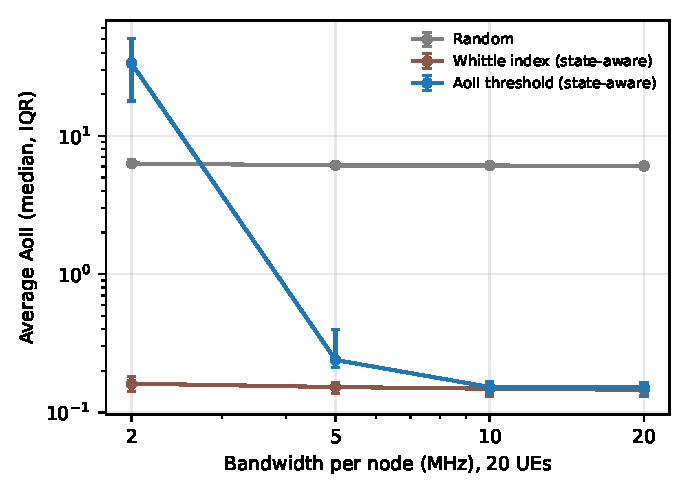
\includegraphics[width=0.8\columnwidth]{figures/capacity_average_aoii.pdf}
\caption{Median average AoII (IQR over 30 seeds) of the per-slot state-aware policies at 20 UEs as the bandwidth per
node is reduced. The Whittle-index scheduler and the AoII-threshold policy coincide while capacity does not bind
and separate below 5~MHz, where uncoordinated threshold transmissions collapse the shared links.}
\label{fig:capacity}
\end{figure}

\textbf{Whittle index and capacity.} At the bandwidths of Table~\ref{tab:simulation_parameters} a node delivers 19 to
40 simultaneous equal sharers within one slot, so capacity never binds and the Whittle scheduler makes the same
decisions as the threshold policy; their AoII is identical to three decimals at every size and in every topology
($p\ge0.18$), and the threshold baseline of this paper is the Whittle-index policy of this regime. Fig.~\ref{fig:capacity}
reduces the bandwidth per node at 20 UEs. At 5~MHz the threshold policy is 57\% worse than the index scheduler
(0.239 against 0.152, $p=4\times10^{-9}$), and at 2~MHz its simultaneous transmissions collapse every shared link
(median AoII 33.5, delivery ratio 0.16) while the capacity-aware index scheduler stays at 0.16. SENTINEL's dedicated
bandwidth levels avoid this regime by construction. The index scheduler's one weakness is the ground-only
deployment, where its admission rule never attempts a node that cannot deliver at the nominal rate and the
threshold policy's blind attempts occasionally succeed on a fading upswing (81 against 63).

%-----------------------------------------------------------------------
\subsection{Validation Against the Exact Minimax Optimum}
\label{sec:exact_validation}
%-----------------------------------------------------------------------

Table~\ref{tab:optimality_gap} reports the mean gap to the exact ILP optimum of $\mathscr{P}_3$ over
capacity-feasible schedules (10 seeds; 5 for the QAOA rows), for the XY-mixer QAOA on the statevector simulator, for
the full distributed pipeline of Algorithm~1 with the compact QUBO and with the epigraph encoding of our earlier
version, and for greedy association refined by local search.
\begin{table}[!t]
\centering
\caption{Mean Optimality Gap (\%) Above the Exact ILP Optimum of $\mathscr{P}_3$}
\label{tab:optimality_gap}
\footnotesize
\resizebox{\columnwidth}{!}{%
\begin{tabular}{|l|c|c|c|c|c|}
\hline
\textbf{Setting} & \textbf{Qubits/domain} & \textbf{XY-QAOA} & \textbf{Compact ADMM} & \textbf{Epigraph ADMM} & \textbf{Greedy+LS} \\
\hline
4--8 UEs, 2+2 & 8--24 & 0.0 (15/15 optimal) & 0.0 & 38--51 & 0.0 \\
10 / 25 UEs, 2+2 & 44 / 78 & -- & 0.0 & 42.7 / 1.8 & 0.0 \\
50 UEs, 4+3 & 142 & -- & 11.5 & 38.8 & 6.0 \\
75 / 100 UEs & 159 / 205 & -- & 49.9 / 60.5 & -- & 14.4 / 11.5 \\
Severity sweep, 20 UEs & 29--66 & -- & 0.0 & 0.2--4.7 & 0.0 \\
$L=1/3/5/6$, 20 UEs & 60--77 & -- & 0.0/3.2/6.9/0.0 & 74/233/9.0/3.8 & 0/0/1.1/0 \\
\hline
\end{tabular}%
}
\end{table}
The XY-mixer QAOA returned the exact optimum on every instance whose domains fit the simulator (8 to 24 qubits),
with 100\% of samples one-hot and capacity-feasible; the epigraph encoding, run with the same classical search, is 38
to 51\% above the optimum on the same instances with 133 to 193 qubits, and a plain simulated annealer on its penalty
landscape found no feasible assignment in 50 solves at 10 UEs. The compact distributed pipeline is exact through 25
UEs and within 12\% at 50; its limit at 75 to 100 UEs is the coordination of five shared satellites among six to eight
domains, which neither more ADMM rounds nor smaller dual steps resolve, and where greedy association with local
search stays within 11 to 14\%. Candidate pruning with $\kappa=4$ never changed the optimum. The exact reference was
solved to proven optimality in under a second on every instance up to 75 UEs and reached its time limit on one in ten
instances at 100 UEs.

%-----------------------------------------------------------------------
\subsection{Quantum Resources and Device Results}
\label{sec:device}
%-----------------------------------------------------------------------

Table~\ref{tab:hardware} lists the transpiled circuits of the hardware-sized domains (depth 1, greedy warm start,
optimization level 3, eight routing trials) and the results of sampling them on the \texttt{ibm\_kingston} and
\texttt{ibm\_fez} processors (Heron r2, 156 qubits, 27 and 28 October 2026; job identifiers in the repository).
Every scenario weight, ADMM target, and QAOA angle was optimized on the simulator; each device job executed only the
final sampling circuit of one or two domains with 4096 shots, and the campaign used 47~s of processor time. The
38-qubit domain exceeds the statevector simulator and received the angles of the largest simulated domain of its run,
relying on the concentration of QAOA parameters across instances~\cite{Brandao2018}. On the FakeTorino and FakeFez
noise models the 18- and 20-qubit domains of the first instance kept 52 and 33\%, and 70 and 48\%, of their shots
feasible, bracketing the device values.
\begin{table}[!t]
\centering
\caption{Transpiled Circuits ($\kappa=4$, depth 1, greedy start) and Device Sampling Results (4096 shots)}
\label{tab:hardware}
\footnotesize
\resizebox{\columnwidth}{!}{%
\begin{tabular}{|l|c|c|c|l|c|c|}
\hline
\textbf{Instance} & \textbf{Dom.} & \textbf{Qubits} & \textbf{2q gates / depth} & \textbf{Device} & \textbf{Feasible shots} & \textbf{Best = opt.} \\
\hline
6 UEs, s1 & 0 & 18 & 139 / 187 & \texttt{ibm\_kingston} & 63.3\% & yes \\
6 UEs, s1 & 1 & 20 & 301 / 428 & \texttt{ibm\_kingston} & 42.7\% & yes \\
6 UEs, s2 & 0 & 18 & 139 / 187 & \texttt{ibm\_kingston} & 60.9\% & yes \\
6 UEs, s2 & 1 & 12 & 58 / 76 & \texttt{ibm\_kingston} & 73.5\% & yes \\
6 UEs, s3 & 0 & 24 & 305 / 387 & \texttt{ibm\_kingston} & 34.8\% & yes \\
6 UEs, s3 & 1 & 14 & 120 / 187 & \texttt{ibm\_kingston} & 69.6\% & yes \\
6 UEs, s5 & 0 & 12 & 58 / 74 & \texttt{ibm\_kingston} & 75.9\% & yes \\
6 UEs, s5 & 1 & 12 & 58 / 74 & \texttt{ibm\_kingston} & 76.4\% & yes \\
6 UEs, s6 & 0 & 8 & 38 / 77 & \texttt{ibm\_fez} & 86.5\% & yes \\
6 UEs, s6 & 1 & 16 & 79 / 77 & \texttt{ibm\_fez} & 61.8\% & yes \\
6 UEs, s7 & 0 & 12 & 58 / 76 & \texttt{ibm\_fez} & 71.9\% & yes \\
6 UEs, s7 & 1 & 18 & 142 / 171 & \texttt{ibm\_fez} & 59.4\% & yes \\
10 UEs, s1 & 0 & 38 & 606 / 626 & \texttt{ibm\_kingston} & 2.6\% & yes \\
\hline
\end{tabular}%
}
\end{table}

Device noise breaks the one-hot structure or the capacity of a part of the shots, which the decoder discards. In all
thirteen domains the best surviving sample equals the noiseless optimum, and every decoded network schedule attains
the exact ILP optimum of its instance. The feasible-shot fraction is the honest measure of the noise: 60 to 86\% at 8
to 18 qubits with up to 139 two-qubit gates, 35 to 43\% at 20 to 24 qubits with about 300 gates, and 2.6\% at 38
qubits with 606 gates. At the 38-qubit scale the device still contains the optimum among 4096 shots, but a few hundred
more two-qubit gates would leave fewer than one feasible shot in a thousand, which places the present limit of the
quantum step at about ten UEs per domain at depth 1. Error suppression does not move it: re-sampling the 24- and
38-qubit domains in one calibration session with dynamical decoupling (XY4)~\cite{Viola1999}, and with dynamical
decoupling plus Pauli twirling~\cite{Wallman2016}, lowered the feasible fraction from the in-session control values of
25.0\% and 2.4\% to 21.1\% and 0.7\%, and to 13.8\% and 0.2\%; these circuits have almost no idle time, so decoupling
pulses add gate error without cancelling idle dephasing, and twirling inserts further single-qubit gates. The best
sample equalled the optimum in every one of those runs. The unmitigated yield of the same circuit also varied by about
ten points between calibration sessions (34.8\% against 25.0\%), so every device comparison here is made within one
session.

On every hardware-sized domain the greedy assignment is already optimal, and the QAOA layers only concentrate a
constrained sampler: from the $W$ state one layer raises the probability of drawing an optimal assignment from the
uniform 0.22 to 0.28 and two layers to 0.42, independently of the shot count above 128, and from the greedy basis
state the optimum is retained with probability 0.99 at depth 1. We therefore claim no quantum advantage. The instances
on which greedy association is suboptimal, 50 UEs and above in Table~\ref{tab:optimality_gap}, need 140 to 200 qubits
per domain, beyond simulation and beyond the gate budget the feasible-shot fractions above allow on current devices;
whether a sampler at that size concentrates on the optimal set is the question this work leaves open.
